\chapter{Implementácia}
%TODO: pozriet ako niekto iny pisal tuto kapitolu tak rozumne


% Yeah this is something I feel is not discussed enough in the RL research community. Like, even if you use the same exact hyperparameters as a SOTA paper, yours still may not work...RL is so finicky.


Použili sme Jupyter notebook a programovací jazyk Python na implementáciu, a aj na experimenty. V balíku acn-portal je v programovacom jazyku Python implementovaná základná trieda pre infraštruktúru nabíjacej siete a aj základná trieda pre plánovacie algoritmy.

Ak vytvárame novú infraštruktúru nabíjacej siete alebo plánovaci algoritmus, tak vždy nami vytvorené triedy dedia od základných tried v balíku acn-portal.
\section{Model predictive control}
% \section{Optimalizačné metódy}
% Všetky optimalizačné metódy implementujeme v jednej triede nazývanej SortedAlgorithms, ktorá taktiež obsahuje triediace plánovacie algoritmy. Triediace plánovacie algoritmy používajú tieto optimalizačné metódy:

% \begin{enumerate}
%     \item Optimalizačnú metódu lineárneho vyhľadávania. Metóda lineárneho vyhľadávania používame v prípade, ak sieť obsahuje nabíjačky, ktoré nevedia dodávať akékoľvek množstvo energie v stanovenom intervale. Napríklad typ nabíjačky DeadbandEVSE nepodporuje dodávky od 0 do 6 ampérov. \cite{lee2021acnsim}
%     \item  Optimalizačnú metódu zlatého rezu.
% \end{enumerate}


% \begin{figure}[H]
%     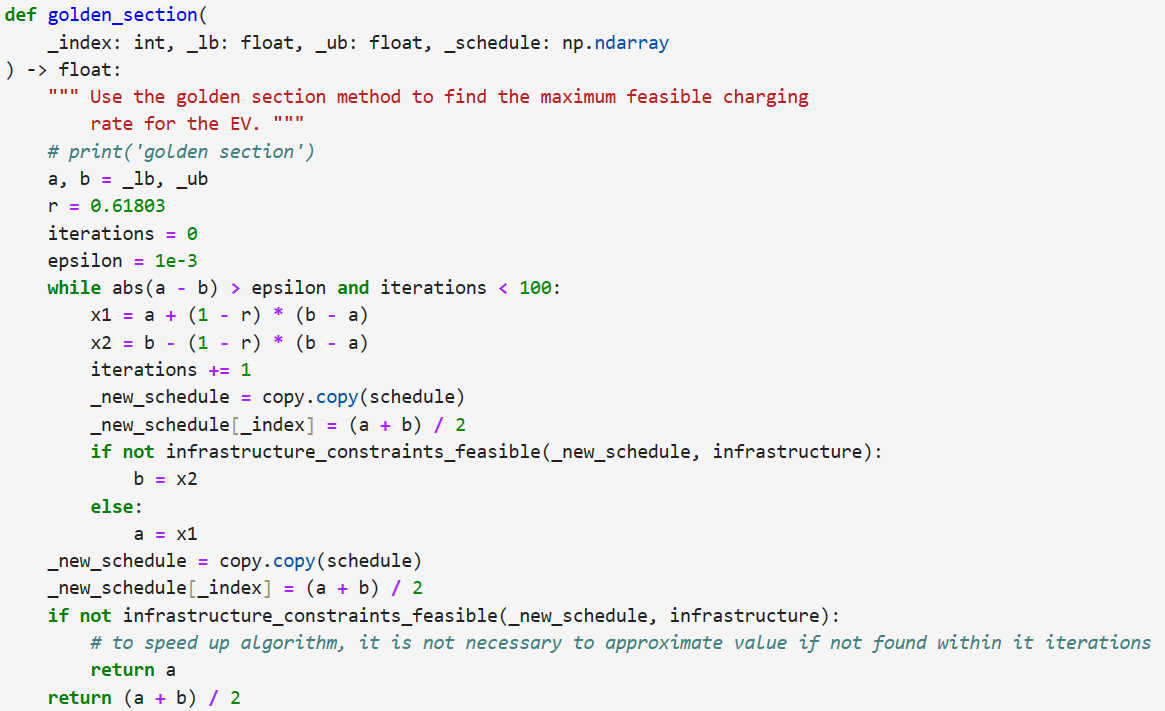
\includegraphics[width=0.8\textwidth]{images/golden_section_code.png}
%     \centering
%     \caption[Kód optimalizačnej metódy zlatého rezu]{Kód optimalizačnej metódy zlatého rezu.}
%     \label{acndata:obr}
%     \end{figure}



% \section{Soft actor critic}


% \begin{verbatim}
%     Initialize neural networks $Q_{}$
%     aa
% \end{verbatim}



% Use simple environments for testing. For discrete control use OpenAI gym classic control’s CartPole. For continuous control use Pendulum. 

% But be careful not to make your algorithm very complex and overfit on these simple problems (i.e use a Massive neural network for policy or value function).

% Rescale environment observations if they have know min max range. Also rescale/clip reward if large.

% Compute useful statistics, such as explained variance (for seeing if your value functions are overfitting), computing KL divergence of policy before and after update (a spike in KL usually means degradation of policy), entropy of your policy.

% Some general neural network tricks are helpful, such as gradient clipping. Not very much so with dropout and batch norm.

% Keep networks simple, no need to use a Massive 20 layer deep resnet architecture.

% Visualize all the above mentioned stats (running mean, std, min, max or episode returns, KL of policy update, explained variance of value functioning fit, network gradients, etc).
% Test for robustness. Try different random seeds, do simple ablation study to see how sensitive your algorithm is to various parameters (learning rate, discount factor, policy entropy constant, etc).
% Last but not least, be patient and don't spend all day looking at your RL algorithm running (it's tempting I know). Write some scripts to automate the experiment steps.



% should i use listing of code or just a picture of code? find out

% \begin{



